\chapter{Introduction}
\section{Structure-based drug discovery principles}
%talking about small drug discovery, not all drug discovery
Small molecule drug design and development is an inventive process of finding new medicines.
This complex task can be divided into smaller $\text{parts}^{\cite{Blass2015BasicDevelopment}}$. 
The first major stage, drug discovery, consists of all the experimental and computational studies designed to move a program from the initial identification of a biological target to the identification of a compound with the potential to be clinically relevant.
This stage can be broken down into several phases:
\begin{enumerate}
    \item \textbf{Target discovery}\\
    One of the key stages is to choose the right target which can be manipulated to influence certain biochemical processes while not affecting the others.
    If the function of the target is defined only hypothetically, the validation is required to understand the link between it and phenotypic traits of the disease of interest.
    
    \item \textbf{Lead discovery}\\
    Once a target has been identified and validated, the biological screening of large libraries of compounds is conducted to discover multiple drug candidates.
    The lead discovery stage will be discussed in more detail further.
    %referencing before labeling
    
    \item \textbf{Lead optimization}\\
    After the initial identification of leads, they can modified chemically to achieve improvements of  affinity, selectivity, mode of action, synthesizability and \acrshort{admet} (\acrlong{admet})-properties.
    Since there are many ways to optimize the compound, this step is cyclic and time-consuming. Finally, the affinity of \glqq original hits\grqq, which is very low, increases by several orders of magnitude.
\end{enumerate}

After lead optimization, several high-potency compounds should be selected as a clinical candidate.

%About the process of choosing for clinical traits

% \begin{figure}[H]
%     \centering
%     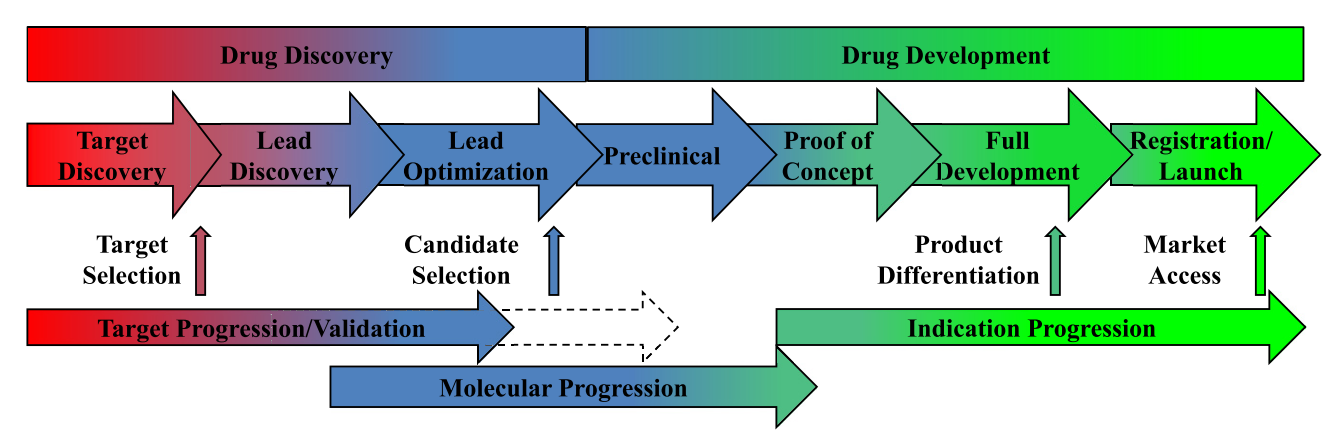
\includegraphics[scale=0.35]{Images/studies.png}
%     \caption{The drug discovery and development process. Taken from \cite{Blass2015BasicDevelopment}.}
%   \label{stud}
% \end{figure}

\begin{figure}
    \centering
    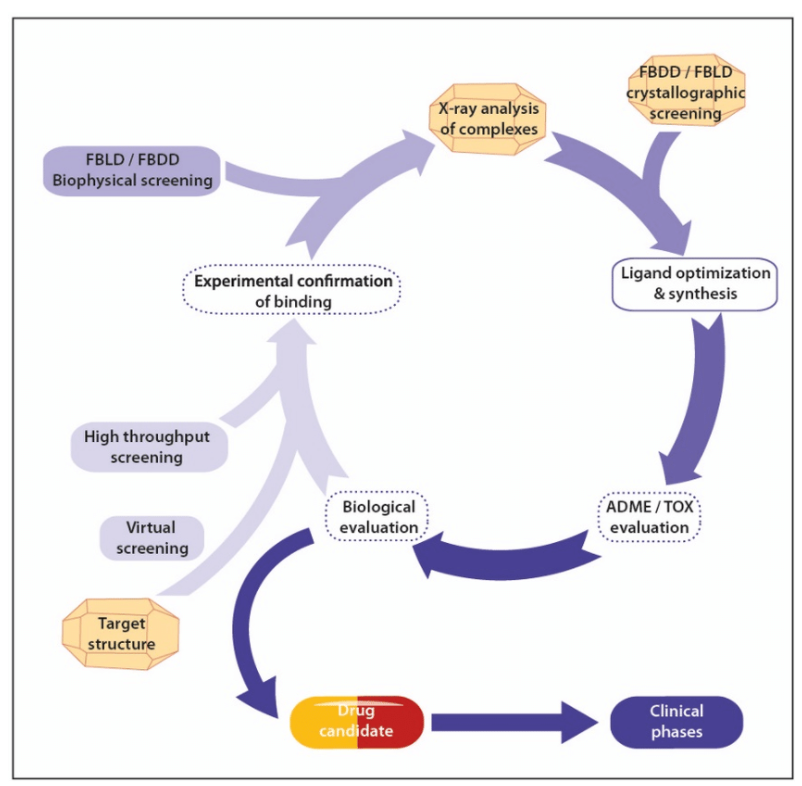
\includegraphics[scale = 0.4]{Images/Maveyraud.png}
    \caption{Drug discovery cycle. Taken from \cite{Maveyraud2020ProteinDiscovery}}
    \label{DrugCycle}
\end{figure}


At the drug discovery stage the potency of the candidate is in the spotlight.
However, high potency is not the only criteria to be examined. 
The second major stage, drug development, is a process of bringing the potential medicine to market.
The candidate must be proven efficient and safe.\\ 

% \begin{enumerate}
%     \item Preclinical studies
%     \item Phase I clinical traits
% \end{enumerate}

\section{Lead discovery stage}%\label{lead_disc}

To identify compounds which can be utilized in clinical setting, two general methods are applied, physical \acrlong{hts} (\acrshort{hts}) and computer-aided drug-design.
Since \acrshort{hts} is expensive and takes more time, money and resources than \textit{in silico }screening, it is common approach to select small subset of molecules from large libraries by means of computational methods - by virtual screening, and after that test them in physical \acrshort{hts}.
The use of computers in drug discovery makes the process of candidate search more quick and cost-efficient.\\

With respect to virtual screening, there are two different techniques: ligand-based and structure-based. The first one uses similarity model
%chemical and pharmacofore similarity
or \acrlong{qsar} (\acrshort{qsar}) to search for possible ligands and needs
%needs what? applied when structure is unknown
Structure-based techniques, in contrast, try to simulate the physics of protein-ligand binding and calculate a quantitative score intended to correlate with the free energy of binding, requiring a target structure but not target-specific bioactivity data.
Structure-based methods include molecular dynamics and computational $\text{docking}^{\cite{Graff2020AcceleratingLearning}}$. Further, \acrshort{qsar} and molecular docking will be considered in detail in this work.\\

\section{Small molecules and databases}

One of the significant questions is where to search candidates for lead discovery stage, as long as chemical space is almost infinite; indeed, it was $\text{estimated}^{\cite{Bohacek1996ThePerspective}}$ that the number of molecules containing 30 heavy atoms (or non-hydrogens) outweighs $10^{60}$.
Usually, potential leads are searched among so called "small molecules".
Currently, this term typically implies an organic compound whose molecular weight is less than roughly 1000 $\text{Da}^{\cite{Gilson2010AnUsers}}$.
Such compounds may be chemically stable and spread through the body to reach a targeted protein after being injected or ingested.
However, molecular weight is not the only criteria for drug-like molecules.
For example, Lipinski's rule  of $5^{\cite{Blass2015BasicDevelopment}}$, suggests that drug-like compounds will have:
\begin{itemize}
    \item a molecular weight lower than 500;
    \item a logP (octanol-water partition coefficient, or lipophilicity) below 5;
    \item less than 5 hydrogen bond donors;
    \item less tan 10 hydrogen bond acceptors;
    \item less than 10 rotatable bonds.
\end{itemize}
Many related rules have been subsequently modified and proposed as the "Rule-of-Three", which defines fragment properties with:
\begin{itemize} 
    \item an average molecular weight $\leq$ 300 Da;
    \item a calculated partition coefficient (Clog P) $\leq$ 3;
    \item the number of hydrogen bond donors $\leq$ 3;
    \item the number of hydrogen bond acceptors $\leq$ 3;
    \item the number of rotatable bonds $\leq$ 3.
\end{itemize}
Also, Pfizer's "Rule of 3/75" has been described which states that compounds with
\begin{itemize}
    \item a ClogP of $\leq$ 3;
    \item topological polar surface area (TPSA) $\ge$ 75
\end{itemize}
have the best chances of being well tolerated from a safety perspective in vivo.
\hfill\break\\
Compounds are gathered in libraries, many of which are freely available online.
The number of purchasable items in these libraries which can be examined in drug design has grown significantly in recent years.
For example, $\text{ZINC20}^{\cite{Irwin2020ZINC20Discovery}}$ is a free database of commercially available compounds that in its current version contains nearly two billions of small molecules, while in $\text{2015}^{\cite{Sterling2015ZINCEveryone}}$ the library comprised roughly 120 million drug-like molecules.
\hfill\break\\
There is a common way to store information about molecules compound libraries.
For example, \acrshort{smiles} notation is often used.\\

\section{\acrshort{qsar} models}
One of the major computational tools in drug design is quantitative structure-activity relationship, \acrshort{qsar} - a method of mapping chemical structure to molecular $\text{properties}^{\cite{Polanski2009ReceptorInteractions}}$. 
Some features, like molecular weight, can be calculated directly for any structure, synthesised or just virtual, while other characteristics, e.g. logP, should be measured only experimentally.
\acrshort{qsar} models attempt to predict these unknown properties based on the information from the molecules which have been already tested experimentally.
Thus, accurate \acrshort{qsar} model can noticeably simplify the compound selection process, providing the information about their biological activity.\\

The history of \acrshort{qsar} modelling started in 1964 with publication of the Hansch's et al. $\text{paper}^{\cite{Hansch1964--Structure}}$ dedicated to correlation between biological activity and chemical structure.
This work was important because of several ideas:
\begin{itemize}

    \item  parameters describing electric, steric and hydrophobic molecular properties had been combined in one equation;
    \item parabolic model for lipophilicity-activity relationship had been proposed based on the reasoning that drug should, on the one hand, circulate in the bloodstream (i.e. be soluble in water), on the other hand, penetrate cell membranes (i.e. dissolve in lipids); 
    \item it had been suggested that logP of a molecule is an additive parameter: the partial contributions of a substituent to the log P of any molecule are almost the same.
\end{itemize}

The introduction of simple \acrshort{qsar} model had played a great role in understanding how molecular structure influences its biological affinity.
The application of the method gave rise to vast amount of publications in wide range of $\text{areas}^{\cite{Debnath2005QuantitativeMillennium}}$: from plant growth regulation and metabolism to cytotoxicity and carciogenicity issues.
\hfill\break\\

Nowadays \acrshort{qsar} modeling is widely practiced in academy, industry, and government institutions around the world.
\acrshort{qsar} models find broad application for assessing potential impacts of chemicals, materials, and nanomaterials on human health and ecological systems.
\hfill\break\\
Considering drug-receptor interaction models, traditional \acrshort{qsar} is receptor-independent, what means that only ligand data is handled.
The main assumption in \acrshort{qsar} is that every property of a molecule is a function of the data derived from its structure.
\hfill\break\\
\section{Molecular descriptors}
  In order to predict chemical properties, a relationship between the property of a molecule and the parameters which characterize its structure should be established.
  To build this property, the molecules' structures should be converted to a convenient, numerical form - molecular descriptors.
  $\text{In the Handbook of Molecular Descriptors}^{\cite{Todeschini2007MethodsChemistry}}$,
  molecular descriptor is defined as the final result of a logic and mathematical procedure which transforms chemical information encoded within a symbolic representation of a molecule into a useful number. \\
%   One of the ways to represent molecules in chemoinformatics is as a vector; then molecules can be interpreted as points in the chemical space; their coordinates are then called descriptors.

\noindent Descriptors should meet several $\text{criteria}^{\cite{
Baskin2020IntroductionChemoinformatics.}}$:
\begin{itemize}
    \item invariant to atom and bonds renumbering;
    \item invariant to rotation and shift;
    \item calculated unambiguously;
    \item easy to operate with: values mustn't be too large or below the machine precision limit;
    \item not a complex number.
\end{itemize}
\hfill\break
Also, it is preferable that descriptor:
\begin{itemize}
    \item can be interpreted physically or structurally;
    \item is not correlated trivially with other descriptors;
    \item does not change significantly due to slightly structure alteration;
    \item is not limited to a small subset of compounds.
\end{itemize}

\noindent Many different types of numerical descriptors are described in the literature. 
Most popular molecular descriptors are 2D-descriptors, which derive from two-dimensional, also called topological, representation of a molecule, which defines the connectivity of atoms in the molecule in terms of the presence and nature of chemical $\text{bonds}^{\cite{Cherkasov2014QSARTo}}$. 

\subsection{Morgan/circular fingerprints}
Also referred as extended-connectivity fingerprints, or $\text{ECFP}^{\cite{Rogers2010Extended-ConnectivityFingerprints}}$.
One of the most common representations in the class of 2D fingerprints, which are computationally inexpensive and easy to interpret and visualize.
The ECFP generation process has three sequential $\text{stages}^{\cite{Rogers2010Extended-ConnectivityFingerprints}}$:
\begin{enumerate}
    \item An initial assignment stage in which each non-hydrogen atom has an integer identifier assigned to it (All rules which are independent of atom numbering can be applied).
    These identifiers are gathered into a fingerprint set. 
    \item An iterative updating stage in which each atom collects its own identifiers among with identifiers of its neighbours (excluding hydrogen atoms) into an array, sorted according to the current identifiers and the order of the bond order (single, double, triple, and aromatic), and a hash function is used to convert this array into a new integer identifier.
    The iteration is repeated a predefined number of times. As the process is repeated, the atom identifier represents a
    substructure of increasing size.
    \item A duplicate identifier removal stage. Structural duplication is a situation when two different atoms contain information about identical structural regions of a molecule.
    The hashed identifier generated for these two atoms will be different, even though they represent the same underlying structure.
    In order to avoid adding useless redundancy to the fingerprint.
    To identify such duplicates, each feature keeps track of the substructure it represents in a molecule.
    Before the newly generated features from an iteration are appended to the fingerprint set, they are checked to see if any structural duplicates exist.
    The removal of duplicates has the additional effect that, at some number of iterations, fewer features will be generated than at the previous iteration level, and at some larger number of iterations, no more new features will be generated.
\end{enumerate}
    Finally, the list of identifiers is folded into a vector (2048-bit by default).
\hfill\break\\
 The ECFP rule for generating initial identifiers is derived from the properties used in the Daylight atomic invariants $\text{rule}^{\cite{Weininger1989SMILES.Notation}}$:
 \begin{itemize}
     \item number of nearest-neighbour non-hydrogen atoms;
     \item number of bonds attached to the atom (not including bonds to hydrogens);
     \item atomic number;
     \item atomic mass;
     \item atomic charge;
     \item number of hydrogens connected to the atom;
     \item is the atom in a ring (1) or not (0) - additional property, not included in Daylight atomic invariants rule.
 \end{itemize}
 To create an integer identifier from this information, these values are hashed into a single 32-bit integer value.\\
 
 Depending on the number of iterations, different names age are given to fingerprints.
 For example, in the RDKit library default number of iterations in the Morgan fingerprints is 2, which corresponds to ECFP4, where 4 represents the \textit{diameter} of the atom environments considered.\\
 
 Different hash functions can be chosen, but should meet special requirements: to map arrays of integers randomly and uniformly into the $2^{32}$-size space of all possible integers; without uniform coverage, the collision rate may increase, leading to a loss of information.

\subsection{Atom pairs fingerprints}
 According to its name, the atom-pair fingerprint is constructed using pairs of atoms (as features) and their topological distances.
 Features used in atom's descriptions contain:
\begin{itemize}
    \item atom's chemical type;
    \item the number of non-hydrogen atoms attached to the it;
    \item the number of bonding $\pi$-electrons that it bears
\end{itemize}
The process of generating atom pair fingerprints consist of several steps:
\begin{enumerate}
    \item Heavy atom are identified and the shortest distance between each pair of them is calculated;
    \item Features of atoms are encoded;
    \item Encoded features are  converted into bit strings and represented as an integer;
    \item Strings are concatenated and passed to a hash function.
\end{enumerate}

\section{Molecular docking}
  Structure-based method, named docking, requires a crystal structure of a target, obtained from NMR, cryo-electron microscopy or X-ray data.
  In principle, docking can screen virtual libraries of great size and diversity, selecting only the best-fitting molecules for synthesis and testing. 
  However, it has serious disadvantage: the technique has a high percentage of false-positive hits. 
  Besides, docking cannot calculate the affinity of compounds $\text{accurately}^{\cite{Lyu2019Ultra-largeChemotypes}}$, still being an effective ranking tool.\\
  
  There are two classes of method needed for docking $\text{implementation}^{\cite{Du2016InsightsMethods}}$: the search algorithm, which is responsible for searching through different orientations, or poses, of a ligand in a binding pocket; and the scoring function, which estimates the binding affinities of poses.\\
  
  Search algorithms must simultaneously be fast and cover chemical space effectively.
  If search space consists of all possible conformations, it is impossible to explore all of it with present computational power; on the contrary, ignoring some degrees of freedom can lead to inaccurate docking results.
  Nowadays, search algorithms can be classified into the following groups of algorithms:
  \begin{itemize}
      \item 
      Rigid-body: both ligand and target are treated as rigid body, and only rotational and transitional freedom is considered;
      \item Flexible-ligand: protein flexibility still doesn't considered, but ligand flexibility does;
      \item Flexible ligand-flexible-protein: both ligand and target are considered as flexible. One of the ways to take into consideration the target flexibility is to dock ligand into multiple fixed receptor $\text{conformations}^{\cite{Totrov2008FlexibleAlternative}}$;
  \end{itemize}
  
  Scoring functions (SF) must predict binding free-energy accurate enough, so different types of physical interactions and entropic effects should be taken into account.
  However, current computational resources constrain the algorithm's complexity.
  Thus, SF make approximations in order to compromise between speed and accuracy. One can divide a wide range of scoring functions into four $\text{classes}^{\cite{Liu2015ClassificationFunctions}, \cite{Li2019AnDocking}}$:
  \begin{itemize}
        \item Empirical methods: the SF sums up the contributions of several terms, each related to energetic factor in protein-ligand binding.
        This terms might be "rewarding", such as hydrogen binding, or "penalties", e.g. frozen rotatable bonds.
        To define coefficients before each term, a regression analysis is conducted with a train set of experimentally determined structures with known binding affinity data.
       \item Physics-based (or force-field based) methods: as well as in empirical methods, binding energy is decomposed into energy terms, but the difference is that physical-based approach fully relies on theory (force field, quantum mechanics and solvent models);
      \item Knowledge-based methods: the approach uses the so-called inverse Boltzmann statistic principle.
      According to Boltzmann statistics, the probability of occurrence of a given state with energy E is proportional to $\exp{(-E/kT)}$, where $k$ is a Boltzmann constant and $T$ is an absolute temperature; thus, the inverse Boltzmann law calculates the energies from the probabilities.
      Hereby, atoms in ligand and target are classified according to their molecular environment; potentials for each pair are derived from inverse Boltzmann analysis of the training dataset, and knowledge-based potential is constructed as a sum of all pairwise potentials.
%       Thus, knowledge-based scoring functions sum pairwise statistical potentials between protein and ligand, wh
%       \begin{equation*}
%           A = \sum_i^{lig} \sum_j^{prot} \omega_{ij}(r),
%       \end{equation*}
%       where 
%       \begin{equation*}
%          \omega_{ij}(r) = -kT \cdot \ln{(g_{ij}(r))} =  -kT \cdot \ln{\frac{\rho_{ij}(r)}{\rho^_{ij}}}
%       \end{equation*}
      \item Descriptor-based (machine learning-based) methods: a relatively new group of algorithms, utilizing \acrshort{qsar} analysis.
      Unlike other types of SF, descriptor-based scoring functions don't have mathematical functional form; they make use of machine-learning algorithms with different types of descriptors used as features. 
  \end{itemize}

Usually, docking is implemented in an exhaustive style: the binding affinities of all molecules in the library are assessed.
Therefore, a considerable part of docking time is spent on working with low-scoring molecules.
The situation is getting worse as docking libraries have been growing exponentially over the past decade; for example, ZINC, a popular database of commercially available compounds for virtual screening contained roughly 1 billion molecules in $2020^{\cite{Irwin2020ZINC20Discovery}}$, which is eight times more than in $2015^{\cite{Sterling2015ZINCEveryone}}$.
With an increase of libraries' sizes, computational costs for screening campaigns have become beyond imagination (e.g.,  475 CPU-years in case of \cite{Gorgulla2020AnScreens}).
Thus, new strategies must be applied to diminish the computational costs in screening campaigns.
One of the possible solutions is to combine classic molecular docking with \acrshort{qsar} modelling in order to remove molecules which are, according to \acrshort{qsar} analysis, less likely to bind the target from screening campaigns.\\

\section{Related works}
% Surprisingly, first works devoted to the docking acceleration, used deep learning (DL) methods without comparing them with less sophisticated models. (\cite{Morrone2020CombiningApproach}, \cite{Jastrzebski2020EmulatingScreening}).\\
 
In a number of works, the construction of an iterative algorithm has been reported.
For instance, Deep $\text{Docking}^{\cite{Gentile2020DeepDiscovery}}$ (DD), a platform which employs \acrshort{qsar} deep models trained on docking scores to iteratively predict the docking outcome for all entities in the library and put away unfavorable molecules, has been presented.
Authors had chosen Morgan fingerprints as features, and had constructed the pipeline in the following way: at initial step, the training subset is docked into the target; in all the rest of the steps, docked molecules are divided into 'hits' and 'non-hits' according to the score cut-off, the DL model is retrained on the received information and predict docking outcomes on the all entities of the library, and the predefined number of molecules selected randomly from predicted 'hits' and docked in order to augment the training set.\\

Another example of iterations usage is a $\text{paper}^{\cite{Graff2020AcceleratingLearning}}$ describing the application of the Bayesian statistics for docking hits search. \\

\begin{landscape}

\begin{longtable}{|l|l|l|l|l|}
\hline
Paper  & Targets and Library & Fingerprints  & Docking software  & ML models  \\ \hline

\begin{tabular}[c]{@{}l@{}}Efficient iterative virtual\\ screening with Apache\\ Spark and conformal\\ $\text{prediction}^{\cite{Ahmed2018EfficientPrediction}}$\end{tabular} &
\begin{tabular}[c]{@{}l@{}}HIV-1 protease, PTPN22, \\ MMP13 and CTDSP1;\\ SureChEMBL (2.2 million)\end{tabular}& 
\begin{tabular}[c]{@{}l@{}}signature \\ molecular\\  descriptor\end{tabular}& 
OEDocking TK & 
\begin{tabular}[c]{@{}l@{}}inductive conformal\\  prediction (ICP)\\  approach with SVM\end{tabular} \\ \hline

\begin{tabular}[c]{@{}l@{}}Deep Docking:\\ A Deep Learning Platform\\ for Augmentation of\\ Structure Based\\ Drug $\text{Discovery}^{\cite{Gentile2020DeepDiscovery}}$ \end{tabular} & 
\begin{tabular}[c]{@{}l@{}}nuclear receptors (AR,\\ ER$\alpha$,  PPAR$\gamma$ ),\\ linases (CAMKK2,\\  CDK6, VEGFR2),\\ GPCRs (ADORA2A, \\ TBXA2R, AT1R),\\ ion channels (Nav1.7, \\ GLIC, GABAA3); ZINC\\ (1.36 billion)\end{tabular}&
\begin{tabular}[c]{@{}l@{}}Morgan\\ (radius 2,\\  size 1024)\end{tabular}&
FRED&
feed-forward NN\\ \hline

\begin{tabular}[c]{@{}l@{}}State of the art iterative\\ docking with logistic\\ regression and Morgan\\ $\text{fingerprints}^{\cite{Martin2021StateFingerprints}}$\end{tabular} &
\begin{tabular}[c]{@{}l@{}}99 million\\ for AmpC,\\ 138 milion\\ for D4\end{tabular}&
\begin{tabular}[c]{@{}l@{}}Morgan\\ (radius 2, \\ size 8192,with\\ pharmacophoric\\ invariants)\end{tabular} & 
DOCK3.7&
logistic regression \\ \hline         
  
\begin{tabular}[c]{@{}l@{}}Lean-Docking:\\ Exploiting Ligands’\\  Predicted Docking \\Scores to Accelerate\\  Molecular $\text{Docking}^{\cite{Berenger2021Lean-Docking:Docking}}$\end{tabular} & 
\begin{tabular}[c]{@{}l@{}} LIT-PCBA data set\\ (15 proteins) \end{tabular}&
\begin{tabular}[c]{@{}l@{}}unfolded counted\\ atom pairs \end{tabular}&
\begin{tabular}[c]{@{}l@{}} CCDC Gold,\\ Glide,\\ AutoDock-Vina,\\FRED ,MOE \end{tabular}&
\begin{tabular}[c]{@{}l@{}}L2-regularized\\ linear support\\ vector regressor\\ (SVR)\end{tabular} \\ \hline

\begin{tabular}[c]{@{}l@{}}Accelerating\\ High-Throughput\\ Virtual Screening\\ Through Molecular\\ Pool-Based\\ Active $\text{Learning}^{\cite{Graff2021AcceleratingLearning}}$ \end{tabular} &
\begin{tabular}[c]{@{}l@{}}thymidylate kinase\\ (PDB ID: 4UNN)\\ AmpC $\beta$-lactamase\\ (PDB ID: 12LS);\\ Enamine10k,\\ Enamine50k\\ HTS collection \\ (2.1 million)\\ for 4UNN\\ ZINC\\ (99 million)\\ for AmpC\end{tabular} &
\begin{tabular}[c]{@{}l@{}}Atom-pair\\ (radius from \\ 1 to 3,\\ size 2048)\end{tabular}&
\begin{tabular}[c]{@{}l@{}}Autodock Vina,\\ DOCK3.7\end{tabular} &
\begin{tabular}[c]{@{}l@{}}random forest,\\ feed-forward NN,\\ directed message \\ passing NN\end{tabular} \\ \hline

\begin{tabular}[c]{@{}l@{}}Efficient Exploration\\ of Chemical Space\\ with Docking and\\ $\text{Deep-Learning}^{\cite{Yang2021EfficientDeep-Learning}}$\end{tabular}&
\begin{tabular}[c]{@{}l@{}}D4 receptor,\\ AmpC $\beta$-lactamase,\\ MT1;\\ 99 million\\ for AmpC,\\ 138 milion\\ for D4,\\ 151 million\\ for MT1\end{tabular} &
\begin{tabular}[c]{@{}l@{}}Morgan\\ (radius 2,\\ size 2048)\end{tabular} &
\begin{tabular}[c]{@{}l@{}}DOCK3.7, \\ Glide SP\end{tabular}&
\begin{tabular}[c]{@{}l@{}}graph-convolutional\\ NN\end{tabular} \\ \hline



\caption{A overview of related papers} \label{rel} \\
\end{longtable}

\end{landscape}